%!TEX root = ../thesis.tex
%*******************************************************************************
%*********************************** First Chapter *****************************
%*******************************************************************************

\chapter{Theoretical Background} % Title of the First Chapter

\ifpdf
\graphicspath{{Chapter2/Figs/Raster/}{Chapter2/Figs/PDF/}{Chapter2/Figs/}}
\else
\graphicspath{{Chapter2/Figs/Vector/}{Chapter2/Figs/}}
\fi

\label{chapter 2}
Following the introductory chapter, where we discussed the fundamental concepts of nuclear fusion and the challenges associated with controlled fusion in tokamaks, we now delve into the theoretical underpinnings necessary to understand the complex dynamics of tokamak operations. Chapter 2 will provide a comprehensive overview of the ideal MHD equations that form the backbone of our theoretical model. We will also explore crucial concepts such as divergence cleaning and the impact of boundary conditions, both hydrodynamic and magnetic, on the behavior of plasma in tokamaks. This foundational knowledge is essential for comprehending the numerical methods and simulations presented in the subsequent chapters.
\section{Ideal MHD Equations}
\label{section2.1}
We are using a magnetohydrodynamics model, which can be regarded as the combined influence of non-magnetic and magnetic fields. Since we are dealing with ideal plasma, the equations governing the non-magnetic field are the Euler equations. They are given as:
\begin{align*}
\frac{\partial \rho}{\partial t} + \nabla \cdot (\rho \mathbf{v}) &= 0 \\
\frac{\partial (\rho \mathbf{v})}{\partial t} + \nabla \cdot \left( \rho \mathbf{v} \otimes \mathbf{v} + \mathbf{I} p \right) &= 0 \\
\frac{\partial E}{\partial t} + \nabla \cdot \left[ \left( E + p \right) \mathbf{v} \right] &= 0
\end{align*}
The variables are the density $\rho$, velocity field $\mathbf{v}$, and internal energy $E$, the pressure $p$. These form the non-magnetic field equations in our MHD model.

The equations governing the magnetic field are Maxwell's equations:
\begin{align*}
\frac{\partial \mathbf{B}}{\partial t} + \nabla \times \mathbf{E} &= 0 \\
\frac{1}{c^2}\frac{\partial \mathbf{E}}{\partial t} + \mu_0 \mathbf{J} - \nabla \times \mathbf{B} &= 0 \\
\nabla \cdot \mathbf{B} &= 0 \\
\nabla \cdot \mathbf{E} &= \frac{\iota}{\epsilon_0}
\end{align*}
Along with Ohm's law:
\begin{align*}
\eta \mathbf{J} = \mathbf{E} + \mathbf{v} \times \mathbf{B}
\end{align*}
and the charge conservation law:
\begin{align*}
\frac{\partial \iota}{\partial t} + \nabla \cdot \mathbf{J} = 0.
\end{align*}
The $\mathbf{B}$ and $\mathbf{E}$ are the vectors of the magnetic field and electric field, respectively. The $\mathbf{J}$ and $\iota$ are the current density and charge density, respectively. The constants are: $c$, the speed of light; $\mu_0=4\pi\times10^{-7}H/m$ the magnetic constant or vacuum permeability; $\epsilon_0$ the vacuum permittivity, where $c^2=1/\mu_0\epsilon_0$. We assume an ideal plasma that is perfectly conductive with no resistivity, $\eta=0$. After ignoring small terms and scaling to counteract the magnetic constant, we rearrange the ideal MHD equations as follows:
\begin{align*}
\frac{\partial \rho}{\partial t} + \nabla \cdot (\rho \mathbf{v}) &= 0 \\
\frac{\partial (\rho \mathbf{v})}{\partial t} + \nabla \cdot \left[ \rho \mathbf{v} \otimes \mathbf{v} + \left( p + \frac{1}{2}\mathbf{B}^2 \right) \mathbf{I} - \mathbf{B} \otimes \mathbf{B} \right] &= 0 \\
\frac{\partial U}{\partial t} + \nabla \cdot \left[ \left( U + p + \frac{1}{2}\mathbf{B}^2 \right) \mathbf{v} - (\mathbf{v} \cdot \mathbf{B}) \mathbf{B} \right] &= 0 \\
\frac{\partial \mathbf{B}}{\partial t} + \nabla \cdot (\mathbf{B} \otimes \mathbf{v} - \mathbf{v} \otimes \mathbf{B}) &= 0
\end{align*}
This represents a homogeneous system without any source terms. In MHD, we use the total energy $U=E+\frac{1}{2}\mathbf{B}^2$ instead. These equations can be rearranged into a two-dimensional form:
\begin{equation}
{{\mathbf{U}}_{t}}+\mathbf{f}_x{{(\mathbf{U})}}+\mathbf{g}_y{{(\mathbf{U})}}=0,
\label{MHDsystem}
\end{equation}
where
\[
\mathbf{U} = \begin{bmatrix}
\rho \\
\rho v_x \\
\rho v_y \\
\rho v_z \\
E \\
B_x \\
B_y \\
B_z 
\end{bmatrix},
\mathbf{f} = \begin{bmatrix}
\rho v_x \\
\rho v_x v_x+p+\frac{1}{2}\mathbf{B}^2-B_x B_x \\
\rho v_x v_y-B_x B_y \\
\rho v_x v_z-B_x B_z \\
v_x(E+p+\frac{1}{2}\mathbf{B}^2)-B_x (v_x B_x + v_y B_y+ v_z B_z) \\
0 \\
v_x B_y-B_x v_y \\
v_x B_z-B_x v_z
\end{bmatrix}\]
\[
\mathbf{g} = \begin{bmatrix}
\rho v_y \\
\rho v_y v_x-B_y B_x \\
\rho v_y v_y+p+\frac{1}{2}\mathbf{B}^2-B_y B_y\\
\rho v_y v_z-B_y B_z \\
v_y(E+p+\frac{1}{2}\mathbf{B}^2)-B_y (v_x B_x + v_y B_y+ v_z B_z) \\
v_y B_x-B_y v_x \\
0 \\
v_y B_z-B_y v_z
\end{bmatrix}
.\]
Setting $\mathbf{B}=0$ results in the Euler system. Theoretically, these equations ensure that the magnetic field's divergence remains zero if it is zero initially. However, numerical methods can introduce errors that violate this condition, necessitating additional techniques.
\section{Divergence Cleaning}
\label{section 2.2}
The last equation of MHD in ~\ref{section2.1} comes from the first equation in Maxwell's equations, Faraday's law:
$$\frac{\partial \mathbf{B}}{\partial t} + \nabla \times \mathbf{E} = 0.$$
Since the operators $\nabla\cdot\left(\nabla\times\mathbf{\phi}\right)\equiv0$ for any vector field $\mathbf{\phi}$, $$\frac{\partial\left(\nabla\cdot\mathbf{B}\right)}{\partial t}=\nabla\cdot\frac{\partial \mathbf{B}}{\partial t}=-\nabla\cdot\left(\nabla\times\mathbf{E}\right)=0.$$
This means that as long as the initial data satisfies the divergence-free condition for the magnetic field, so will the subsequent simulations. However, errors due to numerical multidimensional discretization will lead to the violation of the divergence-free condition \cite{vides2013divergence}. There are methods for better numerical approximation, including divergence cleaning and constrained transport.
Divergence cleaning tries to solve the non-zero divergence after it is produced. There are mainly three kinds of divergence cleaning: hyperbolic, parabolic, and elliptic. A Generalized Lagrange Multiplier (GLM) divergence cleaning method is proposed by Dedner \textit{et al.} \cite{dedner2002hyperbolic}. This method can be hyperbolic, parabolic, or a mixed divergence cleaning depending on the operator \cite{vides2013divergence}. The GLM method introduces a scalar potential $\psi$ for non-vanishing divergence and evolves it to mitigate the non-zero divergence. The system can be evolved in the last MHD equations in ~\ref{section2.1}:
\begin{align*}
\frac{\partial \mathbf{B}}{\partial t} + \nabla \cdot (\mathbf{B} \otimes \mathbf{v} - \mathbf{v} \otimes \mathbf{B}) + \nabla \psi = 0\\
D(\psi) + \nabla \cdot \mathbf{B} = 0
\end{align*}
This system can also evolve as an additional system with only $\mathbf{B}$ and $\psi$ without the $ \nabla \cdot (\mathbf{B} \otimes \mathbf{v} - \mathbf{v} \otimes \mathbf{B})$ term. Specifically, by removing that term in the above equations, the remaining form a set of equations with only $\mathbf{B}$ and $\psi$ independently. Such equations can be updated independently after the iteration of MHD equations in the numerical scheme. $D(\psi)$ is the key operator. For hyperbolic divergence cleaning \cite{vides2013divergence},  $$D(\psi) = \frac{1}{c_h^2} \frac{\partial \psi}{\partial t},$$ which forms a hyperbolic PDE, wave equation, for $\psi$ analytically: 
\begin{align*}
\frac{\partial^2\psi}{\partial t^2}-c_h^2\Delta\psi=0.
\end{align*}
For a parabolic divergence cleaning,$$D(\psi) = \frac{1}{c_p^2} \psi,$$
which form a parabolic PDE, heat equation, for $\psi$ analytically as:
\begin{align*}
\frac{\partial\psi}{\partial t}-c_p^2\Delta\psi=0.
\end{align*}
A mixture of hyperbolic and parabolic operators gives :
\begin{align*}
D(\psi) = \frac{1}{c_h^2} \frac{\partial \psi}{\partial t} + \frac{1}{c_p^2} \psi\\
\end{align*}
In the wave equation for $\psi$, as demonstrated by Tricco \textit{et al.} \cite{tricco2016constrained}, hyperbolic divergence spreads out the non-zero divergence as waves. This method propagates divergence errors very quickly, but dissipated errors still exist globally \cite{tricco2016constrained}. The parabolic one forms a heat equation for $\psi$. The divergence errors are damped and counteracted locally, similar o heat diffusion. Parabolic divergence cleaning effectively eliminates the divergence, but it takes time. Combining their advantages, dissipating and damping, a mixed divergence cleaning is better than either \cite{vides2013divergence,tricco2016constrained}. GLM divergence cleaning is well-used among the community. There are many usages and improvements on it. (i.e. Dellar \cite{dellar2022hyperbolic} adjusts the relaxation time and the behaviour changes from parabolic to hyperbolic. Tricco \textit{et al.} \cite{tricco2016constrained} improve this under smoothed particle magnetohydrodynamics.) Further, there is an elliptic divergence cleaning method \cite{neilsen2006relativistic,cheong2022extension}. This method solves a Possion equation and enforce divergence-free condition after each iteration: 
\begin{align*}
    \nabla^2\psi=\nabla\cdot\mathbf{B}^*, \quad \quad \mathbf{B}^{n+1}=\mathbf{B}^*-\nabla\psi.
\end{align*}
Elliptic divergence cleaning is as effective as the mixed approach. However, it is computationally intensive and consume more computational resources.

In terms of constrained transport methods, they vary, like upwind constrained transport \cite{londrillo2004divergence} and staggered mesh constrained transport \cite{vides2013divergence}. The common idea of constrained transport is to prevent divergence errors from generating except for machine round off errors. For example, staggered mesh constrained transport \cite{vides2013divergence} defines the magnetic field on the cell interfaces, the electric fields at the zone edges under a finite element scheme. In general, constrained transport methods avoid divergence from beginning and no extra computational consumption but they rely on meshes. Furthermore, even when they try to generate errors, slight errors are still generated. In such casees, they are not designed to fix those errors.

In conclusion, divergence cleaning methods represent approaches to evolve a potential to solve non-zero divergences. The hyperbolic method is fast but not clean enough; the parabolic method is slow but eliminating; the elliptic method is efficient but resource-consuming. Constrained transport methods try to avoid the errors from the beginning. Compared with divergence cleaning methods, although they have no extra fixing procedures and accumulate fewer errors, they rely on meshing. Constrained transport methods are not flexible with adaptive meshes.

In our project to simulate the ideal plasma under tokamak vessels, given the ease of implementation, we employ a mixed divergence cleaning approach for eliminating divergence errors in the magnetic field.



\section{Boundary Conditions}
\label{section2.3}
A tokamak vessel looks like a donuts, as well as its magnetic field toroidally and poloidally, as demonstrated in  Figure~\ref{fig:TokamakDonut}. This is designed so that toroidal magnetic field accelerate the plasma while poloidal magnetic field created by the motion of plasma further confine the plasma itself in the core. There are also some equipments like limiters and divertor as shown in Figure \ref{fig:LimiterDivertor}. When we simulate the plasma within the vessel, we take a vertical slice from either side. In that slice, a skewed vertical ellipse fixed rigid body is formed for the plasma to settle into. In computational models, a level set method \cite{andrew2000level} is used to define a boundary. On the boundary, we will need some boundary conditions to model. These boundary conditions can be regarded as a combination of hydrodynamic effects and magnetic effects 
\begin{figure}[H]
    \centering
    \begin{minipage}{0.49\textwidth}
  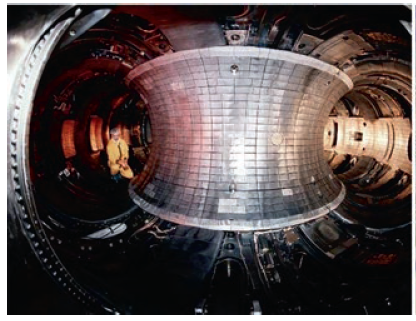
\includegraphics[width=\textwidth]{TokamakVessel.png}
\end{minipage}
\begin{minipage}{0.49\textwidth}
  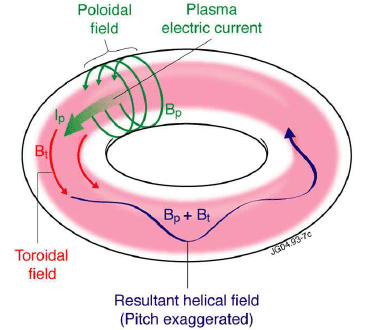
\includegraphics[width=\textwidth]{Toroidal-magnetic-field-B-t.png}
\end{minipage}
    \caption[Donut-shaped Tokamak and magnetic field]{Donut-shaped Tokamak along with toroidal and poloidal. In such device, plasma is confined and accelerated by a toroidal magnetic field just surrounding the 'donut' penetrating from its hole. Then plasma travel along the 'donut' in circle. The motion of ions in plasma forms another poloidal magnetic field further confine them within the core of the elliptic shape of a vertical slice. The 'donut-shaped' is designed in purposes. The right-hand image shows the  The images is adopted from \cite{moynihan2023fusion} and \cite{twarog2011test}. }
    \label{fig:TokamakDonut}
\end{figure}
\begin{figure}
    \centering
    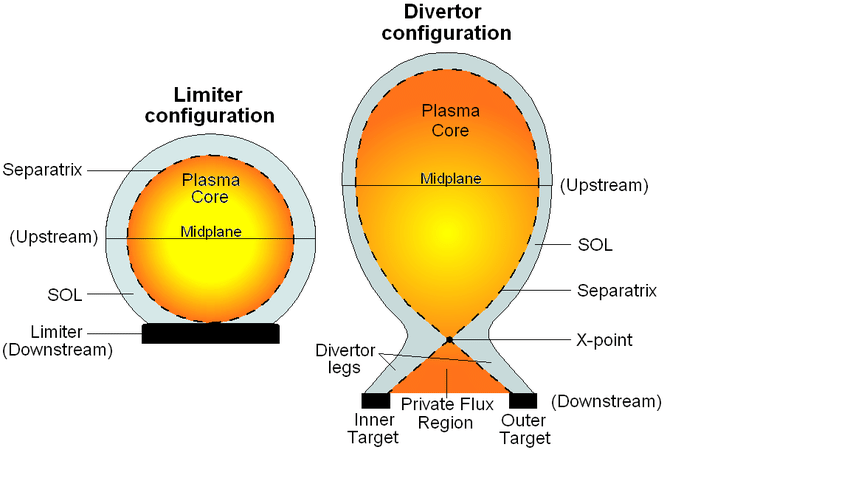
\includegraphics[width=0.5 \textwidth]{Chapter2/Figs/limiter_and_divertor.png}
    \caption[Limiter and divertor in tokamaks]{Limiter and divertor in tokamaks. They are used to protect the walls from plasma erosion. This plot is adopted from \cite{kumar2021analysis}.}
    \label{fig:LimiterDivertor}
\end{figure}


\subsection{Hydrodynamic Effects}
\label{section2.3.1}
In the Euler system without a magnetic field, we apply the reflective boundary condition \cite{sambasivan2009ghost} on the rigid body. Given $\mathbf{v}$ is the velocity vector of the plasma and $\mathbf{U}$ is the velocity vector of the rigid body. We are analyzing on a boundary point with a unit normal vector $\mathbf{n}$. For a normal velocity, it should obey the no-penetration:
$$v_n=U_n.$$ The $v_n=\mathbf{v}\cdot\mathbf{n}$ and $U_n=\mathbf{U}\cdot\mathbf{n}$ are the normal velocities of the plasma and the rigid body on the boundary. For a fixed rigid body $U_n=0$. In a two-dimensional system, the tangential velocity should obey a slip condition:$$\partial v_t /\partial \mathbf{n} =0$$ or a no-slip condition: $$v_t =U_t,$$where $v_t$ and $U_t$ are the tangential components and $\partial v_t /\partial \mathbf{n}$ is its partial derivative . Since the viscosity of ideal plasma is zero, we mainly apply the slip condition. 

Such boundary conditions can be described as Neumann type conditions or Dirichlet type conditions \cite{arendt2004dirichlet}. For a variable $\phi$, they are 
\begin{align*}
    \text{Neumann boundary condition: } \quad &\partial \phi/\partial \mathbf{n} =constant \quad&\text{on boundary}\\
     \text{Dirichlet boundary condition: } \quad&\phi =constant \quad&\text{on boundary}
\end{align*}
To be specific, when we have set value of a variable on boundary, it satisfies the Dirichlet condition; when we have a normal derivative on boundary, it satisfies Neumann condition. Hence, tangential velocity with slip condition satisfies the Neumann boundary condition and normal velocity with no-penetration condition satisfies the Dirichlet condition. The other scalar variables in the Euler system also satisfy the Neumann condition with zero derivative along the normal vector, $\partial \cdot/\partial \mathbf{n}=0$.

\subsection{Magnetic Effects}
There are mainly three kinds of boundary conditions for the magnetic field: perfect conducting wall, insulating wall, and resistive wall.
\subsubsection{Perfect Conducting Wall}
A necessary condition for a perfect conductor is \cite{yanagisawa1991fixed,ju2023incompressible}: $$\mathbf{n}\times\mathbf{E}=0.$$ This is because on a perfect conductor, there is no electric potential difference. According to Faraday's law, the first equation in Maxwell's equations in section~\ref{section2.1}, $\frac{\partial \mathbf{B}}{\partial t} + \nabla \times\mathbf{E} = 0$. Since we are dealing with a fixed rigid body, a normal vector on the boundary is not a function of $t$, $\partial \mathbf{n}/\partial t=0$. Furthermore, $\mathbf{n}\cdot\left(\nabla\times\mathbf{E}\right)=\nabla\cdot\left(\mathbf{n}\times\mathbf{E}\right)=0$. We have an inner product for Faraday's Law:
$$\mathbf{n}\cdot(\frac{\partial \mathbf{B}}{\partial t} + \nabla \times\mathbf{E})=\frac{\partial \left(\mathbf{n}\cdot\mathbf{B}\right)}{\partial t}= 0.$$
This means that on the perfect conducting boundary, normal component of magnetic field only depends on the initial values, given $B_n=\mathbf{B}\cdot\mathbf{n}=B_{n0}$. This forms a 'no-penetration' condition \cite{clauser2021iter} for the normal magnetic field similar to the normal velocity in section ~\ref{section2.3.1}. A perfect conductor will not affect the tangential magnetic field $B_t$. A 'slip' condition is also preserved in the tangential field. In this condition, the normal magnetic field satisfies the Dirichlet boundary condition $B_n=B_{n0}$, and the tangential field satisfies the Neumann boundary condition $\partial B_t/\partial \mathbf{n}=0$.
\subsubsection{Insulating Wall}
An insulator means that no induced magnetic field will be generated inside it. Hence, the magnetic field should be a constant vector along the normal vector. A mathematical description \cite{freidberg2014ideal} for an insulator is:
\begin{align*}
\nabla \times \mathbf{B} &= 0 \\
\nabla \cdot \mathbf{B} &= 0.
\end{align*}
In this situation, both the normal and tangential components of the magnetic field satisfy the Neumann boundary condition $\partial B_t/\partial \mathbf{n} = \partial B_n/\partial \mathbf{n} = 0$.
\subsubsection{Resistive Wall}
A resistive wall can be regarded as an intermediate state between a perfect conducting wall and an insulating wall. A perfect conductor equivalently has infinite conductivity or zero resistivity, while an insulator equivalently has zero conductivity or infinite resistivity. A resistive wall lies in between, with finite conductivity and finite resistivity. The magnetic field is fully reflected by a perfect conducting wall and easily penetrates an insulator. However, with finite resistivity, it penetrates a resistive wall slowly \cite{bondeson2003physics}. The larger the resistivity, the more the penetration. Modeling a resistive wall is inherently more complex than modeling a perfect conductor or an insulator. The preliminary results in this report are all using a perfect conducting wall. Simulations with resistive walls will be considered in the next part of this project and included in the next report.
\subsubsection{Actual Boundary on Tokamak}
The most ideal boundary is the perfect conducting wall. The fully induced reflected magnetic field provides a strong force of passive feedback for stabilizing the plasma \cite{takeda1991computation,clauser2021iter,bondeson2003physics,yolbarsop2022analytic,bondeson1994stabilization}. Between the core plasma and the wall, the outside fixed rigid body, there is sparse plasma with much lower density, which can be regarded as a vacuum \cite{clauser2021iter,takeda1991computation}. As long as the perfect conducting wall is close enough to the plasma, it remains stable. This vacuum region can be regarded as an insulator. Both models of a fixed perfect conducting wall and a vacuum free boundary space are used in computational models of tokamak devices \cite{clauser2021iter,freidberg2014ideal}. However, the actual walls of tokamaks have finite conductivity. A more realistic scenario replaces the perfect conducting wall with a resistive wall \cite{clauser2021iter}. The resistivity reduces the model's stability, where the external modes start to grow \cite{haney1989variational,bondeson2003physics,bondeson1994stabilization}. A resistive plasma further increases the modeling complexity \cite{yolbarsop2022analytic}.

Our project mainly models the ideal plasma with no resistivity and viscosity under a perfect conducting fixed rigid body and then generalizes it to a resistive model.